\documentclass[final,3p]{elsarticle}

\usepackage[T1]{fontenc}
\usepackage[utf8]{inputenc}
\usepackage{mathptmx}
\usepackage{microtype}
\usepackage{amsmath,amssymb}
\usepackage{graphicx}
\usepackage{booktabs}
\usepackage{multirow}
\usepackage{array}
\usepackage{tabularx}
\usepackage[table]{xcolor}
\usepackage{tikz}
\usetikzlibrary{positioning,arrows.meta,fit,calc,backgrounds,shapes.geometric}
\usepackage{algorithm}
\usepackage[noend]{algpseudocode}
\usepackage{enumitem}
\setlist{nosep,leftmargin=*}
\usepackage[hidelinks]{hyperref}
\usepackage[capitalise,nameinlink]{cleveref}
\crefname{algorithm}{Algorithm}{Algorithms}
\crefname{equation}{Eq.}{Eqs.}
\crefname{line}{line}{lines}

\definecolor{ink}{HTML}{0B0B0B}
\definecolor{muted}{HTML}{52514E}
\definecolor{band}{HTML}{F0EFEC}
\definecolor{accent}{HTML}{2A78D6}
\definecolor{warm}{HTML}{EB6834}
\newcommand{\ci}[2]{\scriptsize[#1, #2]}
\algrenewcommand\algorithmicrequire{\textbf{Input:}}
\algrenewcommand\algorithmicensure{\textbf{Output:}}
\algnewcommand{\LineComment}[1]{\State \textcolor{muted}{\(\triangleright\) #1}}
\DeclareMathOperator*{\topk}{top\text{-}k}
\DeclareMathOperator{\AUC}{AUC}
\DeclareMathOperator{\BCE}{BCE}
\DeclareMathOperator{\GAP}{GAP}

\renewcommand{\topfraction}{0.9}
\renewcommand{\bottomfraction}{0.8}
\renewcommand{\textfraction}{0.07}
\renewcommand{\floatpagefraction}{0.75}
\setcounter{topnumber}{3}
\setcounter{totalnumber}{5}

\journal{Computers in Biology and Medicine}

\begin{document}

\begin{frontmatter}

\title{Adversarial deconfounding with pseudo device labels does not remove the device shortcut in pneumothorax detection: a pre-registered, multi-seed external evaluation of twelve models}

\author{Yazan Aljeroudi\corref{cor1}}
\ead{yazan.aljeroudi@gmail.com}
\cortext[cor1]{Corresponding author.}
\affiliation{organization={[Affiliation to be added]}}

\begin{abstract}
\textbf{Background:} Pneumothorax classifiers trained on public chest radiographs can learn to detect the \emph{treatment} (a chest tube or other visible device) rather than the air. We tested, under a pre-registered protocol, whether a model trained to be insensitive to devices detects \emph{untreated} pneumothorax better on external data than current methods.

\textbf{Methods:} Models were developed on SIIM-ACR (10{,}675 radiographs). Because the planned development set with chest-tube masks (CANDID-PTX) was inaccessible, a pre-registered amendment replaced tube labels with ``visible device'' pseudo-labels from a classifier trained only on the training split of an external NIH-derived device cohort. The proposed model combined a gradient-reversal device adversary with segmentation-based top-$k$ mask pooling on a U-Net with an EfficientNet-B4 encoder. It was compared with three ablations, two sensitivity variants and six re-trained baselines (U-Net ResNet34, SegFormer-B2, Group DRO, an auxiliary device classifier, RAD-DINO linear probe and fine-tuned) in 54 training runs (3--5 seeds each). The primary external set was the NIH cohort's released test split with human device labels (521 images; 125 pneumothorax, 36 without a device); PTX-498 (482 positives, three hospitals) was secondary. The protocol was frozen before external data were opened, and each model was evaluated once.

\textbf{Results:} The proposed model did not outperform any baseline on the primary endpoints: its untreated sensitivity at the transferred threshold was 0.22 versus 0.28 for the best baseline, its untreated AUROC was the lowest of all models (0.70, 95\% CI 0.58--0.81, versus 0.76--0.82) and its device-minus-untreated AUROC gap was the largest (0.26, 95\% CI 0.15--0.37, versus 0.08--0.18). All twelve models showed a positive gap, and in eight the pneumothorax score itself separated device-bearing from device-free \emph{negatives} (AUROC 0.56--0.71). Training curves show the adversary was driven to chance on the development data while device information remained recoverable from the same features externally (probe AUROC 0.90).

\textbf{Conclusions:} Adversarial removal of a noisy, pseudo-labelled device attribute did not reduce, and appeared to increase, reliance on devices. The shortcut is present in every architecture tested, including a radiology foundation model. Untreated-stratum performance should be reported routinely for pneumothorax models.
\end{abstract}

\begin{keyword}
Pneumothorax \sep Chest radiography \sep Shortcut learning \sep Domain-adversarial training \sep External validation \sep Pre-registration \sep Negative result
\end{keyword}

\end{frontmatter}

%% ============================================================ INTRODUCTION
\section{Introduction}
\label{sec:intro}

Deep learning systems for chest radiographs often exploit features that correlate with a label in the training data but are not the pathology itself \citep{geirhos2020shortcut,zech2018variable,degrave2021covid,badgeley2019hip,banerjee2023shortcuts}. Pneumothorax is a clear example. Many radiographs labelled positive in public datasets were taken \emph{after} treatment, so they show a chest tube. A model can reach a high overall AUROC by detecting the tube, and then fail on the patients who matter most: those whose pneumothorax has not yet been recognised and treated \citep{oakdenrayner2020hidden,taylor2018pneumothorax,rueckel2020tubes}. Pooled estimates suggest that pneumothorax detectors match physicians \citep{sugibayashi2023meta,katzman2024meta}, but most primary studies carry a high risk of bias and few report performance stratified by treatment status.

Two families of methods are commonly used to reduce such shortcuts. Domain-adversarial training removes information about a nuisance attribute from the representation by gradient reversal \citep{ganin2015dann,kim2019learning,zhao2020confounder}. Group distributionally robust optimisation (Group DRO) up-weights the worst-performing group defined by label and attribute \citep{sagawa2020groupdro}. A third, architectural idea is to derive the image-level score from the segmentation of the air itself, so that evidence outside the pneumothorax region cannot drive the decision \citep{rueckel2021annotations}.

We designed a study to test whether combining these ideas yields a detector of untreated pneumothorax that is better than current methods on external data. To avoid the analytic flexibility that inflates positive results, all endpoints, pass thresholds, baselines, ablations and statistical tests were pre-registered and frozen before any external test set was opened \citep{nosek2018prereg}. The original design relied on CANDID-PTX \citep{feng2021candid}, the only public dataset we know of with chest-tube segmentation masks. Access could not be obtained; the dataset is reported to be unavailable outside Health New Zealand since February 2024. We therefore executed a pre-registered amendment (``Plan B'') that uses pseudo-labelled visible devices in place of chest tubes.

This paper reports the result: a clear negative. We present it in full because (i) it is informative for anyone applying adversarial deconfounding with proxy labels, (ii) the same experiment provides a controlled, multi-seed audit of the device shortcut across twelve models, including a radiology foundation model \citep{perezgarcia2025raddino}, and (iii) it documents a failure of threshold transfer between two public pneumothorax datasets.

\paragraph{Contributions}
\begin{itemize}
  \item A pre-registered, frozen-before-testing evaluation of a device-deconfounded pneumothorax model against six re-trained baselines and five ablation and sensitivity variants (54 training runs), each evaluated once on external data (\cref{sec:design,sec:system}).
  \item A precise specification of the model, training step, scoring rule and decision procedure (\cref{alg:pseudo,alg:train,alg:score,alg:eval,alg:boot}).
  \item Evidence that gradient-reversal removal of a pseudo-labelled device attribute \emph{increased} the device--untreated gap on external data, with training dynamics that explain why (\cref{sec:res-endpoints,sec:res-conv}).
  \item A cross-architecture audit showing a device shortcut in every model and device information inside the pneumothorax score itself (\cref{sec:res-shortcut,sec:res-qual}).
  \item Open code, split files, per-image predictions and all 54 checkpoints.
\end{itemize}

%% ============================================================ RELATED WORK
\section{Related work}
\label{sec:related}

\paragraph{Chest tubes as a confounder in pneumothorax detection}
\citet{rueckel2020tubes} showed on 6{,}434 annotated supine radiographs that thoracic tubes are strong confounders: comparing untreated positives with tube-bearing negatives removed the discriminative power of two public-data algorithms. \citet{rueckel2021annotations} reduced this bias by adding in-image annotations of the visceral pleural line to training. Saliency analyses of vision transformers and CNNs trained on public data revealed a strong bias toward tubes \citep{wollek2023attention}. \citet{jimenez2023shortcuts} released drain annotations for a subset of NIH ChestX-ray14 pneumothorax images and confirmed the shortcut. More recently, \citet{sourget2025clip} found that six CLIP-based chest radiograph models all performed worse on pneumothorax without drains, and \citet{li2025featurequality} reported that medical foundation-model encoders, RAD-DINO among them, use chest tubes as a shortcut for pneumothorax classification. The shortcut is not universal. \citet{thian2021external} found no difference between tube-present and tube-absent radiographs across six external sites, \citet{seah2021hidden} found a commercial model non-inferior in the intercostal-drain subgroup, and \citet{graf2020tube} reported comparable performance with and without tubes after lung segmentation and patch classification. Other shortcuts, such as exposure parameters, can also dominate pneumothorax predictions \citep{shu2026exposure}.

\paragraph{Mitigation with attribute labels}
Adversarial and disentanglement methods remove a known confounder from the representation \citep{ganin2015dann,kim2019learning,zhao2020confounder}. In chest radiography they have been used for view position in pneumonia \citep{janizek2020adversarial}, source dataset in COVID-19 \citep{robinson2022disentangle} and race \citep{correa2023cav}. Benchmarks show that such methods help mainly under strong spurious correlation and that latent-space analyses reveal differences that classification metrics miss \citep{muller2026disentangle}. Group DRO optimises the worst group \citep{sagawa2020groupdro}, but reweighting can be problematic when bias is not the only cause of poor performance \citep{kumar2023droinvariant}. For pneumothorax specifically, \citet{bandaru2026untreated} added auxiliary chest-tube detection to improve untreated classification.

\paragraph{Mitigation without attribute labels}
When attribute labels are missing, they can be inferred. JTT up-weights examples an initial model misclassifies \citep{liu2021jtt}; pseudo bias-balanced learning predicts per-sample bias labels for chest radiographs \citep{luo2022pbbl}. Worst-group accuracy with inferred groups still trails that with oracle groups, which motivated more precise group inference \citep{han2024gic}. Our design sits between these settings: device labels were inferred by a separately trained classifier, then used as if they were true attribute labels. Counterfactual image editing is a further, data-centric route \citep{cooke2026roentmod}.

\paragraph{Evaluation practice}
Shortcut reliance is often invisible in overall metrics and is more prevalent than reported \citep{unnikrishnan2024pest,vasquez2024cleverhans}. Removing a shortcut in-distribution does not guarantee better behaviour out of distribution \citep{yang2024limits}, and foundation models can encode unwanted attributes \citep{glocker2023foundation}. Saliency maps are an unreliable basis for localisation claims \citep{saporta2022saliency,arun2021saliency}. We therefore rely on stratified external metrics and a score-level device test, and use saliency only as illustration.

\Cref{tab:related} positions this study against the pneumothorax-specific literature.

\begin{table}[!tbp]
\centering\scriptsize
\setlength{\tabcolsep}{3pt}
\caption{Pneumothorax studies that examined chest tubes or devices. ``Strat.'' = performance reported by device status; ``Mitig.'' = a method aimed at reducing device reliance. Findings are summarised from the cited abstracts.}
\label{tab:related}
\begin{tabularx}{\linewidth}{@{}p{2.3cm} p{3.1cm} c c X@{}}
\toprule
Study & Data (test) & Strat. & Mitig. & Main finding on devices \\
\midrule
\citet{rueckel2020tubes} & 6{,}434 supine CXRs, single centre & \checkmark & --- & Tubes are strong confounders; untreated vs tube-bearing negatives removes discrimination \\
\citet{rueckel2021annotations} & 3{,}062 supine CXRs & \checkmark & \checkmark & Pleural-line annotations raise AUROC and reduce tube bias \\
\citet{graf2020tube} & Public benchmark & \checkmark & \checkmark & Lung segmentation + patch classification; comparable with/without tubes \\
\citet{thian2021external} & Six external sites & \checkmark & --- & No difference with vs without chest tube \\
\citet{seah2021hidden} & 2{,}557 studies, AU/US & \checkmark & --- & Commercial model non-inferior in drain subgroup \\
\citet{feng2022triage} & CANDID-PTX & --- & --- & Grad-CAM: negligible confounding reported \\
\citet{jimenez2023shortcuts} & NIH-CXR14 subset & \checkmark & --- & Drain annotations released; shortcut confirmed \\
\citet{wollek2023attention} & CXR14, VinBigData, SIIM & --- & --- & Saliency reveals strong tube bias \\
\citet{sourget2025clip} & MIMIC, CXR14, NEATX & \checkmark & --- & Six CLIP models worse without drains \\
\citet{li2025featurequality} & Eight foundation encoders & \checkmark & --- & Foundation models use tube shortcut \\
\citet{bandaru2026untreated} & Public data & \checkmark & \checkmark & Auxiliary tube detection for untreated cases \\
\rowcolor{band}\textbf{This study} & NIH device cohort (521), PTX-498 (482) & \checkmark & \checkmark & Pre-registered; 12 models; adversarial debiasing enlarged the gap; shortcut in all models \\
\bottomrule
\end{tabularx}
\end{table}

%% ============================================================ METHODS
\section{Materials and methods}
\label{sec:methods}

\subsection{Study design and pre-registration}
\label{sec:design}
The protocol (\texttt{PREREGISTRATION.md} in the code repository) fixed hypotheses, datasets and roles, the operating point, primary and secondary endpoints, ablations, baselines and statistics. Amendment~1 (Plan B) was added on 23 September 2026, before any external evaluation, when CANDID-PTX access proved unavailable. Deviations were recorded on 24 September 2026, again before freezing. The frozen file's SHA-256 hash was written to the repository, and the external-evaluation script refuses to run if the file changes. External test sets were opened once per trained model. \Cref{fig:design} summarises the design. Reporting follows the spirit of CLAIM and TRIPOD+AI \citep{mongan2020claim,collins2024tripodai}.

\begin{figure}[!tbp]
\centering
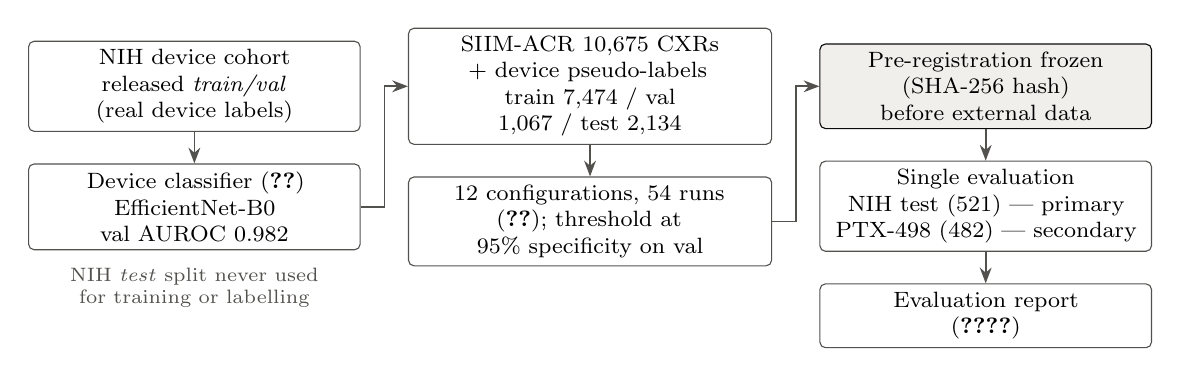
\begin{tikzpicture}[
  node distance=4mm and 6mm,
  box/.style={draw=muted, rounded corners=2pt, align=center, font=\footnotesize, inner sep=3pt, text width=#1},
  box/.default=4.4cm,
  hl/.style={box=#1, fill=band, draw=ink},
  hl/.default=4.4cm,
  arr/.style={-{Stealth[length=2mm]}, draw=muted, line width=0.6pt}]
\node[box=4.0cm] (nihtr) {NIH device cohort\\ released \emph{train/val}\\ (real device labels)};
\node[box=4.0cm, below=of nihtr] (dev) {Device classifier (\cref{alg:pseudo})\\ EfficientNet-B0\\ val AUROC 0.982};
\node[box=4.4cm, right=of nihtr] (siim) {SIIM-ACR 10{,}675 CXRs\\ + device pseudo-labels\\ train 7{,}474 / val 1{,}067 / test 2{,}134};
\node[box=4.4cm, below=of siim] (train) {12 configurations, 54 runs\\ (\cref{alg:train}); threshold at\\ 95\% specificity on val};
\node[hl=4.0cm, right=of siim] (freeze) {Pre-registration frozen\\ (SHA-256 hash)\\ before external data};
\node[box=4.0cm, below=of freeze] (ext) {Single evaluation\\ NIH test (521) --- primary\\ PTX-498 (482) --- secondary};
\node[box=4.0cm, below=of ext] (acc) {Evaluation report\\ (\cref{alg:eval,alg:boot})};
\draw[arr] (nihtr) -- (dev);
\draw[arr] (dev.east) -- ++(3mm,0) |- (siim.west);
\draw[arr] (siim) -- (train);
\draw[arr] (train.east) -- ++(3mm,0) |- (freeze.west);
\draw[arr] (freeze) -- (ext);
\draw[arr] (ext) -- (acc);
\node[font=\scriptsize, text=muted, below=1mm of dev, text width=4.0cm, align=center] {NIH \emph{test} split never used for training or labelling};
\end{tikzpicture}
\caption{Study design (Plan B). Device pseudo-labels for SIIM-ACR come from a classifier trained only on the NIH cohort's released training split and thresholded on its validation split. External test sets were opened once, after the pre-registration was frozen.}
\label{fig:design}
\end{figure}

\subsection{System architecture}
\label{sec:system}
All computation ran through a single, versioned pipeline (\cref{fig:system}). The code repository holds the source, configuration files, fixed split files and the frozen protocol. Cloud GPU pods (one NVIDIA A40 or L40S each) start from a public PyTorch image, clone the repository with a token held as a platform secret, and run a stage queue defined in \texttt{configs/experiments.yaml}: \emph{data} (download and conversion), \emph{planb\_prep} (device pseudo-labels, \cref{alg:pseudo}), \emph{planb\_gate1} (pilot on development validation only), \emph{planb\_main\_a/b} (one entry per model and seed, \cref{alg:train}, split over two pods) and \emph{planb\_gate2} (freeze, leakage check and single external evaluation, \cref{alg:score,alg:eval,alg:boot}). Each finished run pushes its configuration, training log, per-epoch validation metrics and per-image predictions back to the repository; checkpoints are uploaded as release assets. Several pods trained in parallel. Concurrent pushes were reconciled by rebasing, and a failed run was logged and skipped without stopping the queue. A pod stops itself when its queue is empty or its time budget is spent. The external evaluation script checks the protocol hash before opening any external set and writes a single evaluation report. The 54 checkpoints, with a manifest of SHA-256 checksums and decision thresholds and a model card, are deposited on Zenodo (record 22966372; DOI 10.5281/zenodo.22966372).

\begin{figure}[!tbp]
\centering
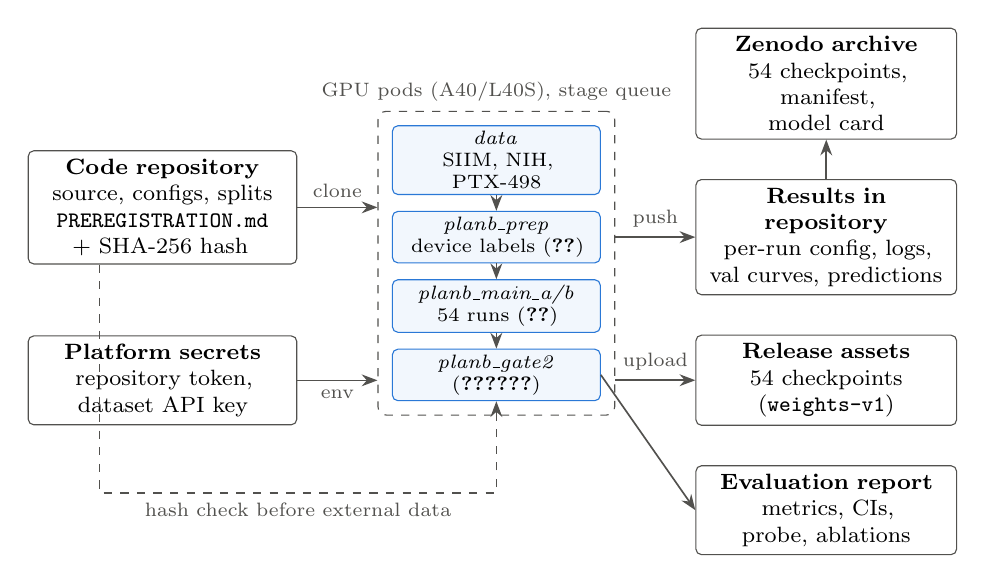
\begin{tikzpicture}[
  node distance=5mm and 7mm,
  box/.style={draw=muted, rounded corners=2pt, align=center, font=\footnotesize, inner sep=3pt, text width=#1, fill=white},
  box/.default=3.3cm,
  st/.style={draw=accent, rounded corners=2pt, align=center, font=\scriptsize, inner sep=2pt, text width=2.5cm, fill=accent!6},
  arr/.style={-{Stealth[length=2mm]}, draw=muted, line width=0.6pt},
  lab/.style={font=\scriptsize, text=muted}]
\node[box=3.2cm] (repo) {\textbf{Code repository}\\ source, configs, splits\\ \texttt{PREREGISTRATION.md}\\ + SHA-256 hash};
\node[box=3.2cm, below=9mm of repo] (secrets) {\textbf{Platform secrets}\\ repository token,\\ dataset API key};
\node[st, right=12mm of repo, yshift=6mm] (s1) {\emph{data}\\ SIIM, NIH, PTX-498};
\node[st, below=2mm of s1] (s2) {\emph{planb\_prep}\\ device labels (\cref{alg:pseudo})};
\node[st, below=2mm of s2] (s3) {\emph{planb\_main\_a/b}\\ 54 runs (\cref{alg:train})};
\node[st, below=2mm of s3] (s4) {\emph{planb\_gate2}\\ (\cref{alg:score,alg:eval,alg:boot})};
\begin{scope}[on background layer]
\node[draw=muted, dashed, rounded corners=3pt, fit=(s1)(s4), inner sep=5pt, label={[lab]above:GPU pods (A40/L40S), stage queue}] (pod) {};
\end{scope}
\node[box=3.1cm, right=12mm of s2] (res) {\textbf{Results in repository}\\ per-run config, logs,\\ val curves, predictions};
\node[box=3.1cm, below=5mm of res] (rel) {\textbf{Release assets}\\ 54 checkpoints\\ (\texttt{weights-v1})};
\node[box=3.1cm, below=5mm of rel] (rep) {\textbf{Evaluation report}\\ metrics, CIs,\\ probe, ablations};
\node[box=3.1cm, above=5mm of res] (zen) {\textbf{Zenodo archive}\\ 54 checkpoints, manifest,\\ model card};
\draw[arr] (repo.east) -- node[lab, above, sloped]{clone} (pod.west |- repo.east);
\draw[arr] (secrets.east) -- node[lab, below, sloped]{env} (pod.west |- secrets.east);
\draw[arr] (s1) -- (s2); \draw[arr] (s2) -- (s3); \draw[arr] (s3) -- (s4);
\draw[arr] (pod.east |- res.west) -- node[lab, above]{push} (res.west);
\draw[arr] (pod.east |- rel.west) -- node[lab, above]{upload} (rel.west);
\draw[arr] (s4.east) -- (rep.west);
\draw[arr] (res) -- (zen);
\draw[arr, dashed] (repo.south) ++(-0.8,0) -- ++(0,-2.9) -| node[lab, pos=0.25, below]{hash check before external data} (s4.south);
\end{tikzpicture}
\caption{System architecture. Every stage runs from the versioned repository on disposable GPU pods; results flow back to the repository, checkpoints to release assets. The evaluation stage verifies the frozen protocol hash before opening external data.}
\label{fig:system}
\end{figure}

\subsection{Data}
\label{sec:data}
\Cref{tab:data} lists the datasets and their roles, and \cref{fig:examples} shows examples.

\textbf{SIIM-ACR} \citep{siim2019kaggle} (10{,}675 radiographs with labels, 2{,}379 with pneumothorax and segmentation masks) was the development set. It was split 70/10/20 into train (7{,}474), validation (1{,}067) and internal test (2{,}134) with a fixed seed (2026). SIIM-ACR has one identifier per image, so splitting was at image level, with near-duplicates (perceptual hash, Hamming distance $\le 4$) grouped into the same split.

\textbf{NIH device cohort} \citep{zamora2026cohort} is a curated, patient-wise pneumothorax versus no-finding cohort derived from NIH ChestX-ray14 \citep{wang2017chestxray8}. It contains 4{,}388 radiographs (2{,}194 pneumothorax) with human visible-device annotations and a fixed patient-wise split. Its released \emph{test} split (878 images) was the primary external set. Because SIIM-ACR images were also drawn from ChestX-ray14, we removed from this test split every image with a near-duplicate in SIIM-ACR (357 images). This left 521 images: 125 with pneumothorax (89 with a visible device, 36 without) and 396 without (157 with a device, 238 without, 1 unlabelled). The cohort's train and validation splits were used only for the device classifier and a pilot, never for training pneumothorax models.

\textbf{PTX-498} \citep{wang2021ptx498,wang2021deepsdm} (version v2-fix) contains 498 pneumothorax radiographs with masks from three hospitals. After removing 16 near-duplicates of development images, 482 remained. It contains only positives, so it was used for sensitivity, Dice and size endpoints, not for AUROC or specificity.

\begin{table}[!tbp]
\centering\small
\caption{Datasets and roles in the Plan B analysis.}
\label{tab:data}
\begin{tabularx}{\linewidth}{@{}l p{3.6cm} X r@{}}
\toprule
Dataset & Role & Labels used & Images \\
\midrule
SIIM-ACR & Development (train/val/internal test) & Pneumothorax masks; device \emph{pseudo}-labels (\cref{alg:pseudo}) & 10{,}675 \\
NIH device cohort, released test & Primary external & Pneumothorax vs no finding; human visible-device labels & 521 \\
NIH device cohort, released train/val & Device classifier only & Visible device (uncertain excluded) & 2{,}626 / 875 \\
PTX-498 (v2-fix) & Secondary external (positives only) & Pneumothorax masks, 3 sites & 482 \\
\bottomrule
\end{tabularx}
\end{table}

\subsection{Device pseudo-labels}
\label{sec:pseudo}
\Cref{alg:pseudo} specifies the labelling step. An EfficientNet-B0 \citep{tan2019efficientnet} was trained for eight epochs at 384~px on the NIH cohort's training split (2{,}626 images with a certain device label). The epoch with the best validation AUROC was kept, and the cut-off maximising balanced accuracy was chosen on the validation split (875 images). Validation AUROC was 0.982, with sensitivity 0.956 and specificity 0.957 at the cut-off (0.398). Applied to SIIM-ACR, it labelled 62.3\% of images as device-bearing: 86.9\% of pneumothorax-positive and 55.3\% of negative images. ``Untreated'' in SIIM-ACR therefore means ``no device predicted''. In the NIH test set it means ``no visible device'' according to the human annotations.

\begin{algorithm}[!tbp]
\caption{Device pseudo-labelling (stage \emph{planb\_prep})}
\label{alg:pseudo}
\begin{algorithmic}[1]
\Require NIH cohort train split $\mathcal{T}$ and validation split $\mathcal{V}$ with device labels $d\in\{0,1\}$ (uncertain labels removed); SIIM-ACR images $\mathcal{S}$
\Ensure Device pseudo-label $\hat d(x)$ for every $x\in\mathcal{S}$
\State Initialise EfficientNet-B0 $f_\phi$ from ImageNet weights; resize inputs to $384\times384$
\For{$e = 1,\dots,8$}
  \State Train $f_\phi$ one epoch on $\mathcal{T}$ with $\BCE(f_\phi(x),d)$
  \State $a_e \gets \AUC\big(\{d\},\{f_\phi(x)\}\big)$ on $\mathcal{V}$; keep $\phi^\star \gets \phi$ if $a_e$ is the best so far \label{line:pseudo-select}
\EndFor
\State $t^\star \gets \arg\max_t \tfrac12\big(\mathrm{sens}_{\mathcal{V}}(t)+\mathrm{spec}_{\mathcal{V}}(t)\big)$ using $f_{\phi^\star}$ \label{line:pseudo-thr}
\For{each $x\in\mathcal{S}$ (all splits)}
  \State $\hat d(x) \gets \mathbf{1}\big[\sigma(f_{\phi^\star}(x)) \ge t^\star\big]$
\EndFor
\State \Return $\hat d$ \Comment{NIH \emph{test} split is never touched}
\end{algorithmic}
\end{algorithm}

\subsection{Proposed model}
\label{sec:model}
\Cref{fig:arch} shows the network. An input radiograph $x\in\mathbb{R}^{3\times H\times W}$ ($H=W=512$) passes through an EfficientNet-B4 encoder $E$ that returns five feature maps $F_1,\dots,F_5$, and a U-Net decoder $D$ \citep{ronneberger2015unet} with skip connections that returns pixel logits
\begin{equation}
Z = D(F_1,\dots,F_5)\in\mathbb{R}^{H\times W}.
\label{eq:seg}
\end{equation}
Let $h=\GAP(F_5)\in\mathbb{R}^{c}$ be the globally average-pooled deepest feature map ($c=448$ for EfficientNet-B4).

\paragraph{C4: mask pooling}
The image-level logit is computed from the segmentation map alone:
\begin{equation}
s(x) = a\cdot\frac{1}{k}\sum_{(i,j)\in\topk(Z)} Z_{ij} + b,\qquad k=\max\big(1,\lfloor\rho HW\rfloor\big),\ \rho=0.005,
\label{eq:maskpool}
\end{equation}
where $\topk(Z)$ indexes the $k$ largest pixel logits ($k=1{,}310$ at 512~px) and $a,b$ are learned scalars initialised to $1$ and $0$. Without C4, a global head is used instead: $s(x)=w^\top \mathrm{Dropout}(h)+b$.

\paragraph{C2: device adversary}
A gradient-reversal layer $R_\lambda$ \citep{ganin2015dann} is the identity in the forward pass and multiplies gradients by $-\lambda$ in the backward pass:
\begin{equation}
R_\lambda(h)=h,\qquad \frac{\partial R_\lambda(h)}{\partial h}=-\lambda I.
\label{eq:grl}
\end{equation}
A two-layer perceptron $g_\psi$ (256 hidden units, ReLU, dropout 0.2) predicts the device label from $R_\lambda(h)$, giving $\hat d = g_\psi(R_\lambda(h))$. The adversary minimises its loss; because of \cref{eq:grl}, the encoder receives the negated gradient and is pushed to make $h$ uninformative about the device. We used $\lambda=0.1$.

\paragraph{Losses}
For a mini-batch $\mathcal{B}$ with pneumothorax labels $y$, masks $M$ (available for positives) and device pseudo-labels $\hat d$,
\begin{align}
\mathcal{L}_{\text{cls}} &= \tfrac{1}{|\mathcal{B}|}\textstyle\sum_{n}\BCE\big(s(x_n),y_n\big), \label{eq:lcls}\\
\mathcal{L}_{\text{seg}} &= \BCE_{\text{pix}}(Z,M) + \Big(1-\frac{2\sum Z^\sigma M + \epsilon}{\sum Z^\sigma + \sum M + \epsilon}\Big)_{y=1}, \label{eq:lseg}\\
\mathcal{L}_{\text{adv}} &= \tfrac{1}{|\mathcal{B}|}\textstyle\sum_n\BCE\big(g_\psi(R_\lambda(h_n)),\hat d_n\big), \label{eq:ladv}\\
\mathcal{L} &= \mathcal{L}_{\text{cls}} + w_{\text{seg}}\,\mathcal{L}_{\text{seg}} + w_{\text{adv}}\,\mathcal{L}_{\text{adv}},\qquad w_{\text{seg}}=w_{\text{adv}}=1, \label{eq:ltotal}
\end{align}
where $Z^\sigma$ is the sigmoid of $Z$, the pixel BCE is averaged over images that have a mask (empty masks for negatives), and the soft-Dice term is computed over positives only. \Cref{alg:train} gives the full training procedure and \cref{alg:score} the scoring rule.

\begin{figure}[!tbp]
\centering
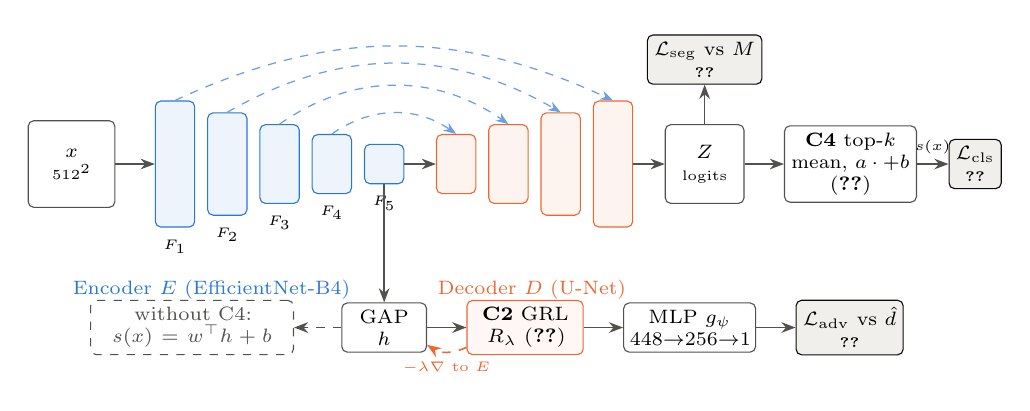
\begin{tikzpicture}[
  node distance=4mm and 5mm,
  blk/.style={draw=muted, rounded corners=2pt, align=center, font=\scriptsize, inner sep=2.5pt, fill=white},
  enc/.style={blk, fill=accent!8, draw=accent, minimum height=#1, minimum width=5mm},
  dec/.style={blk, fill=warm!8, draw=warm, minimum height=#1, minimum width=5mm},
  loss/.style={blk, draw=ink, fill=band, font=\scriptsize},
  arr/.style={-{Stealth[length=1.8mm]}, draw=muted, line width=0.55pt},
  skip/.style={-{Stealth[length=1.6mm]}, draw=accent!70, line width=0.45pt, dashed}]
% input
\node[blk, minimum width=11mm, minimum height=11mm] (x) {$x$\\ \tiny 512$^2$};
% encoder stages
\node[enc=16mm, right=5mm of x] (e1) {};
\node[enc=13mm, right=1.5mm of e1] (e2) {};
\node[enc=10mm, right=1.5mm of e2] (e3) {};
\node[enc=7.5mm, right=1.5mm of e3] (e4) {};
\node[enc=5mm, right=1.5mm of e4] (e5) {};
\node[font=\scriptsize, text=accent] (elab) at ($(e2)+(-0.2,-1.6)$) {Encoder $E$ (EfficientNet-B4)};
\foreach \i in {1,...,5} {\node[font=\tiny, below=0.3mm of e\i] {$F_\i$};}
% decoder
\node[dec=7.5mm, right=4mm of e5] (d4) {};
\node[dec=10mm, right=1.5mm of d4] (d3) {};
\node[dec=13mm, right=1.5mm of d3] (d2) {};
\node[dec=16mm, right=1.5mm of d2] (d1) {};
\node[font=\scriptsize, text=warm] at ($(d3)+(0.3,-1.6)$) {Decoder $D$ (U-Net)};
\draw[arr] (x) -- (e1);
\draw[arr] (e5) -- (d4);
\draw[skip] (e4.north) to[bend left=35] (d4.north);
\draw[skip] (e3.north) to[bend left=35] (d3.north);
\draw[skip] (e2.north) to[bend left=30] (d2.north);
\draw[skip] (e1.north) to[bend left=25] (d1.north);
% seg map
\node[blk, right=4mm of d1, minimum width=10mm, minimum height=10mm] (Z) {$Z$\\ \tiny logits};
\draw[arr] (d1) -- (Z);
% C4
\node[blk, right=5mm of Z, text width=15mm] (tk) {\textbf{C4} top-$k$\\ mean, $a\cdot{+}b$\\ (\cref{eq:maskpool})};
\draw[arr] (Z) -- (tk);
\node[loss, right=4mm of tk] (lcls) {$\mathcal{L}_{\text{cls}}$\\ \tiny \cref{eq:lcls}};
\draw[arr] (tk) -- node[font=\tiny, above]{$s(x)$} (lcls);
\node[loss, above=5mm of Z] (lseg) {$\mathcal{L}_{\text{seg}}$ vs $M$\\ \tiny \cref{eq:lseg}};
\draw[arr] (Z) -- (lseg);
% C2 branch
\node[blk, below=15mm of e5, text width=9mm] (gap) {GAP\\ $h$};
\draw[arr] (e5) -- (gap);
\node[blk, right=5mm of gap, text width=13mm, draw=warm, fill=warm!5] (grl) {\textbf{C2} GRL\\ $R_\lambda$ (\cref{eq:grl})};
\node[blk, right=5mm of grl, text width=15mm] (mlp) {MLP $g_\psi$\\ 448$\to$256$\to$1};
\node[loss, right=5mm of mlp] (ladv) {$\mathcal{L}_{\text{adv}}$ vs $\hat d$\\ \tiny \cref{eq:ladv}};
\draw[arr] (gap) -- (grl); \draw[arr] (grl) -- (mlp); \draw[arr] (mlp) -- (ladv);
\draw[-{Stealth[length=1.8mm]}, draw=warm, line width=0.6pt, dashed] ($(grl.south west)+(0,0.1)$) to[bend left=30] node[font=\tiny, text=warm, below]{$-\lambda\nabla$ to $E$} ($(gap.south east)+(0,0.1)$);
% global head alternative
\node[blk, left=6mm of gap, text width=24mm, draw=muted, dashed, text=muted] (glob) {without C4: $s(x)=w^\top h+b$};
\draw[arr, dashed] (gap.west) -- (glob.east);
\end{tikzpicture}
\caption{Proposed network (C2+C4). The image score is computed from the segmentation logits by top-$k$ mask pooling (C4). A device adversary with gradient reversal (C2) acts on the pooled deepest encoder features $h$. Ablations remove C2, replace C4 by the global head (dashed), or both. Dashed blue arrows are U-Net skip connections.}
\label{fig:arch}
\end{figure}

\begin{algorithm}[!tbp]
\caption{Training one configuration with one seed (stages \emph{planb\_main\_a/b})}
\label{alg:train}
\begin{algorithmic}[1]
\Require SIIM-ACR train $\mathcal{D}_{tr}$, validation $\mathcal{D}_{va}$; device pseudo-labels $\hat d$ (\cref{alg:pseudo}); seed $r$; switches C2, C4, DRO
\Ensure Checkpoint $\theta^\star$ and threshold $\tau$
\State Set all random seeds to $r$; initialise $E$ from ImageNet; $\theta\gets(E,D,a,b,g_\psi)$
\State Sampler with replacement, weights such that positives form 50\% of draws
\State AdamW (lr $3\!\times\!10^{-4}$, weight decay $10^{-4}$), 1-epoch linear warm-up then cosine decay; AMP
\State $u^\star\gets-\infty$; \textbf{if} DRO: $q\gets\mathbf{1}/4$ over groups $(y,\hat d)$
\For{$e=1,\dots,20$}
  \For{each mini-batch $\mathcal{B}$ of 16 from the sampler}
    \State Augment: flip, rotation $\pm10^\circ$, scale $0.9$--$1.1$, shift $\pm5\%$, brightness/contrast
    \State Forward: $Z$ by \cref{eq:seg}; $s$ by \cref{eq:maskpool} if C4, else global head
    \State $\mathcal{L}\gets\mathcal{L}_{\text{cls}}+\mathcal{L}_{\text{seg}}$ \Comment{\cref{eq:lcls,eq:lseg}}
    \If{C2} \State $\mathcal{L}\gets\mathcal{L}+\mathcal{L}_{\text{adv}}$ \Comment{\cref{eq:ladv}; reversal by \cref{eq:grl}} \label{line:adv}
    \EndIf
    \If{DRO} \State replace $\mathcal{L}_{\text{cls}}$ by $\sum_g q_g\ell_g$, then $q_g\gets q_g e^{\eta\ell_g}$, renormalise ($\eta=0.01$) \label{line:dro}
    \EndIf
    \State Backward; clip gradient norm at 5; optimiser and scheduler step
  \EndFor
  \State On $\mathcal{D}_{va}$: $\tau_e\gets$ threshold at 95\% specificity (\cref{eq:tau}); $u_e\gets$ untreated sensitivity at $\tau_e$
  \If{$u_e>u^\star$} \State $u^\star\gets u_e$; $\theta^\star\gets\theta$; $\tau\gets\tau_e$ \label{line:select}
  \EndIf
\EndFor
\State \Return $\theta^\star,\tau$
\end{algorithmic}
\end{algorithm}

\subsection{Ablations and baselines}
\label{sec:baselines}
All pneumothorax models except RAD-DINO use a segmentation network from the Segmentation Models PyTorch library \citep{iakubovskii2019smp} with ImageNet weights and a 512$\times$512 input. \Cref{tab:models} summarises the configurations.

\begin{itemize}
  \item \textbf{Ablations:} C4 only (no adversary); C2 only (global head instead of mask pooling); base (neither). \textbf{Sensitivity runs:} $\lambda=0.01$ and $\lambda=1.0$ with C2 and the global head.
  \item \textbf{Baselines:} U-Net with a ResNet34 encoder \citep{he2016resnet}, a common choice among SIIM-ACR challenge solutions (mask pooling); SegFormer-B2 \citep{xie2021segformer} (mask pooling); Group DRO \citep{sagawa2020groupdro} over four groups (pneumothorax $\times$ device, step size 0.01, \cref{line:dro} of \cref{alg:train}) on the EfficientNet-B4 U-Net; an auxiliary device classifier without gradient reversal (linear head on $h$, loss weight 0.5), after \citet{bandaru2026untreated}; and RAD-DINO \citep{perezgarcia2025raddino} with a linear head on the pooled output at 518~px, either frozen (linear probe; lr $10^{-3}$, batch 32) or fully fine-tuned (lr $2\times10^{-5}$).
\end{itemize}

The planned nnU-Net \citep{isensee2021nnunet} and zero-shot multimodal baselines were not run in Plan B. This was recorded before freezing, and neither enters the ``best baseline'' comparisons. Tube-mask components (inpainting and auxiliary tube segmentation) require tube masks and were dropped.

\begin{table}[!tbp]
\centering\small
\caption{Model configurations. All were trained on the same SIIM-ACR splits with the same augmentation and schedule (\cref{alg:train}). ``Mask pool'' = \cref{eq:maskpool}; ``Global'' = linear head on $h$.}
\label{tab:models}
\begin{tabular}{@{}l l l l c@{}}
\toprule
Model & Backbone & Image score & Device handling & Seeds \\
\midrule
\textbf{Proposed (C2+C4)} & U-Net / EfficientNet-B4 & Mask pool & Gradient reversal, $\lambda$=0.1 & 5 \\
Ablation: C4 only & U-Net / EfficientNet-B4 & Mask pool & --- & 5 \\
Ablation: C2 only & U-Net / EfficientNet-B4 & Global & Gradient reversal, $\lambda$=0.1 & 5 \\
Ablation: base & U-Net / EfficientNet-B4 & Global & --- & 5 \\
Sensitivity $\lambda$=0.01 / 1.0 & U-Net / EfficientNet-B4 & Global & Gradient reversal & 3 / 3 \\
U-Net ResNet34 & U-Net / ResNet34 & Mask pool & --- & 5 \\
SegFormer-B2 & SegFormer / MiT-B2 & Mask pool & --- & 3 \\
Group DRO & U-Net / EfficientNet-B4 & Mask pool & Worst-group reweighting & 5 \\
Aux.\ device classifier & U-Net / EfficientNet-B4 & Global & Auxiliary head (no reversal) & 5 \\
RAD-DINO linear probe & ViT-B (RAD-DINO), frozen & Global & --- & 5 \\
RAD-DINO fine-tuned & ViT-B (RAD-DINO) & Global & --- & 5 \\
\bottomrule
\end{tabular}
\end{table}

\subsection{Training, operating point and scoring}
\label{sec:training}
Training followed \cref{alg:train}: 20 epochs, AdamW (learning rate $3\times10^{-4}$, weight decay $10^{-4}$, batch 16), one epoch of linear warm-up followed by cosine decay, gradient clipping at 5, mixed precision and positive oversampling to 50\% of draws. Augmentation was horizontal flipping, rotation ($\pm10^\circ$), scaling (0.9--1.1), translation ($\pm5\%$) and random brightness/contrast. The checkpoint kept was the epoch with the highest untreated sensitivity at 95\% specificity on SIIM-ACR validation (\cref{line:select}). That set contains only 32 untreated positives, which we discuss as a limitation. Each model's threshold was set at 95\% specificity on the same validation set,
\begin{equation}
\tau = \mathrm{next}\big(v_{(\lceil 0.95\,n_0\rceil)}\big),
\label{eq:tau}
\end{equation}
where $v_{(1)}\le\dots\le v_{(n_0)}$ are the sorted validation scores of the $n_0$ negatives and $\mathrm{next}(\cdot)$ is the next representable number above, and applied unchanged to all other sets (\cref{alg:score}). Runs took about 20--50 minutes each on a single NVIDIA A40.

\begin{algorithm}[!tbp]
\caption{Scoring an image with a trained configuration}
\label{alg:score}
\begin{algorithmic}[1]
\Require Image $x$; checkpoints $\{\theta^\star_r\}_{r=1}^{R}$ and thresholds $\{\tau_r\}$ from \cref{alg:train}
\Ensure Seed-averaged probability $\bar p(x)$ and decision $\hat y(x)$
\For{$r=1,\dots,R$}
  \State Resize $x$ to $512^2$ (RAD-DINO: $518^2$); forward pass with $\theta^\star_r$ in evaluation mode
  \If{mask pooling} \State $s_r\gets a\cdot\mathrm{mean}\big(\topk(Z)\big)+b$ \Comment{\cref{eq:maskpool}}
  \Else \State $s_r\gets w^\top h+b$
  \EndIf
  \State $p_r\gets\sigma(s_r)$ \Comment{the adversary $g_\psi$ is not used at inference}
\EndFor
\State $\bar p(x)\gets\frac1R\sum_r p_r$ \Comment{primary analyses use seed-averaged scores}
\State $\bar\tau\gets$ \cref{eq:tau} applied to seed-averaged SIIM-ACR validation scores\label{line:tau-avg}
\State $\hat y(x)\gets\mathbf{1}[\bar p(x)\ge\bar\tau]$ (primary summaries); per-seed $\mathbf{1}[p_r\ge\tau_r]$ for seed-level analyses
\State \Return $\bar p(x),\hat y(x)$
\end{algorithmic}
\end{algorithm}

\subsection{Endpoints}
\label{sec:endpoints}
The two primary endpoints, both on the NIH test set, were untreated sensitivity at the threshold transferred from SIIM-ACR validation and the device--untreated AUROC gap. Secondary endpoints were untreated AUROC (paired DeLong test with Holm correction across baselines \citep{delong1988,holm1979}), sensitivity for small pneumothorax, Dice, agreement of the predicted size class (weighted $\kappa$), calibration after temperature scaling (15-bin ECE \citep{guo2017calibration}) and seed-to-seed stability. Each was compared with the strongest re-trained baseline for that dataset and metric, chosen from U-Net ResNet34, the C4-only EfficientNet-B4 U-Net, SegFormer-B2, Group DRO, the auxiliary device classifier and both RAD-DINO variants; segmentation endpoints used only the segmentation baselines. \Cref{alg:eval} gives the evaluation procedure. With $P_{\text{dev}}$, $P_{\text{untr}}$ and $N$ the device-present positives, untreated positives and all negatives, the stratified quantities are
\begin{align}
\Delta_{\text{gap}} &= \AUC(P_{\text{dev}},N)-\AUC(P_{\text{untr}},N), \label{eq:gap}\\
\AUC_{\text{dev}\mid y=0} &= \Pr\big[\bar p(x^{+})>\bar p(x^{-})\big],\quad x^{+}\in N_{\text{dev}},\ x^{-}\in N_{\text{none}}, \label{eq:devscore}
\end{align}
where $\AUC(A,B)$ is the probability that a random member of $A$ scores above a random member of $B$ (ties count one half). \Cref{eq:gap} is a primary endpoint. \Cref{eq:devscore}, the \emph{device-in-score} AUROC, is exploratory: a value above 0.5 means that a device alone raises the pneumothorax score in images without pneumothorax.

\paragraph{Device probe, leakage audit and ablations}
\emph{Device probe:} 5-fold logistic regression predicting the device label from each model's pooled features on the NIH test set, as a measure of residual device information. \emph{Leakage audit:} patient overlap across development splits and perceptual-hash near-duplicates between any training-like split and any test split. \emph{Ablations:} each component was removed in turn, and untreated sensitivity on the NIH test set was compared with the full model using paired seeds and the seed-averaged difference with a bootstrap CI.

\begin{algorithm}[!tbp]
\caption{Single external evaluation (stage \emph{planb\_gate2})}
\label{alg:eval}
\begin{algorithmic}[1]
\Require Frozen protocol file $\Pi$ and stored hash $H$; all trained runs; external sets NIH test, PTX-498
\Ensure Per-image predictions and the evaluation report
\If{$\mathrm{SHA256}(\Pi)\neq H$} \State \textbf{abort} \Comment{no external data opened} \label{line:hash}
\EndIf
\State Run leakage audit (patients, perceptual-hash near-duplicates across all splits)
\For{each run} \State score every external image once with \cref{alg:score}; store predictions
\EndFor
\State Compute primary and secondary endpoints for every model, with CIs from \cref{alg:boot}
\State Untreated AUROC: paired DeLong test vs each baseline, Holm correction
\State Calibration: fit temperature on SIIM-ACR validation, then 15-bin ECE on NIH
\State Device probe on pooled features; paired-seed ablation comparisons
\State \Return predictions and report
\end{algorithmic}
\end{algorithm}

\begin{table}[!tbp]
\centering\small
\caption{Primary and secondary endpoints for the proposed model and the strongest re-trained comparator for each endpoint. Primary external set = NIH test. Differences are proposed minus comparator with 95\% patient-cluster bootstrap CIs.}
\label{tab:endpoints}
\begin{tabularx}{\linewidth}{@{}>{\raggedright\arraybackslash}p{5.2cm} >{\raggedright\arraybackslash}p{3.4cm} >{\raggedright\arraybackslash}X@{}}
\toprule
Endpoint & Proposed & Strongest comparator; difference \\
\midrule
\multicolumn{3}{@{}l}{\emph{Primary (NIH test)}}\\
Untreated sensitivity, transferred threshold & 0.222 & SegFormer-B2 0.278; $-$0.056 \ci{$-$0.143}{0.000} \\
Device--untreated AUROC gap (\cref{eq:gap}) & 0.258 & Group DRO 0.086 (smallest gap) \\
\midrule
\multicolumn{3}{@{}l}{\emph{Secondary}}\\
Untreated AUROC (NIH) & 0.695 & RAD-DINO probe 0.816; $-$0.121, DeLong $p_\text{Holm}=0.046$ \\
Small-pneumothorax sensitivity & SIIM 0.636; PTX-498 0.404 & SIIM 0.693 ($n$=225); PTX-498 0.634 ($n$=161) \\
Dice & SIIM 0.460; PTX-498 0.478 & SegFormer-B2: SIIM 0.499; PTX-498 0.731 \\
Size class, weighted $\kappa$ & SIIM 0.375; PTX-498 0.478 & --- \\
ECE after temperature scaling (NIH) & 0.097 ($T$=1.56) & --- \\
Seed SD of untreated sensitivity & 0.070 & 0/5 seeds above the comparator mean \\
\bottomrule
\end{tabularx}
\end{table}

\subsection{Statistics}
\label{sec:stats}
Primary analyses use seed-averaged scores. 95\% CIs come from a patient-cluster bootstrap with 2{,}000 resamples (\cref{alg:boot}). Paired differences between models use the same resamples, so that between-model correlation is preserved. Pneumothorax size follows the British Thoracic Society rim criterion ($\ge$20~mm) where pixel spacing is known, and area-fraction tertiles otherwise \citep{macduff2010bts}.

\paragraph{Exploratory analyses (not pre-registered)} On the NIH test set we computed, for all twelve configurations, AUROC for untreated and for device-present positives against all negatives; paired differences between the proposed model and each comparator; the device-in-score AUROC (\cref{eq:devscore}); sensitivity at 95\% specificity recalibrated on the NIH set itself (an oracle threshold); an analysis excluding images involved in the leakage finding; per-epoch training and validation curves (\cref{sec:res-conv}); and seed-averaged segmentation maps and Grad-CAM \citep{selvaraju2020gradcam} for examples chosen by fixed rules (\cref{sec:res-qual}). These results are descriptive.

\begin{algorithm}[!tbp]
\caption{Patient-cluster bootstrap for CIs and paired differences}
\label{alg:boot}
\begin{algorithmic}[1]
\Require Test images with patient IDs; seed-averaged scores $\bar p^{(m)}$ for every model $m$; statistic $T$ (e.g.\ \cref{eq:gap,eq:devscore}); $B=2000$
\Ensure Point estimates and 95\% CIs for $T^{(m)}$ and for $T^{(\text{prop})}-T^{(m)}$
\State Group image indices by patient: $\mathcal{C}_1,\dots,\mathcal{C}_K$; fix the random generator (seed 0)
\State $\hat T^{(m)}\gets T\big(\bar p^{(m)}\big)$ on all images
\For{$b=1,\dots,B$}
  \State Draw $K$ patients with replacement; $I_b\gets$ concatenation of their image indices
  \For{each model $m$} \State $T^{(m)}_b\gets T\big(\bar p^{(m)}[I_b]\big)$ \Comment{same $I_b$ for all models}
  \EndFor
  \State $\delta^{(m)}_b\gets T^{(\text{prop})}_b-T^{(m)}_b$
\EndFor
\State Drop undefined replicates (e.g.\ a stratum absent from $I_b$)
\State \Return $\hat T^{(m)}$, percentiles 2.5/97.5 of $\{T^{(m)}_b\}$ and of $\{\delta^{(m)}_b\}$
\end{algorithmic}
\end{algorithm}

%% ============================================================ RESULTS
\section{Results}
\label{sec:results}

\subsection{Primary and secondary endpoints}
\label{sec:res-endpoints}
All 54 runs completed. The proposed model did not improve on the strongest comparator for any endpoint (\cref{tab:endpoints}). On the NIH test set its untreated sensitivity at the transferred threshold was 0.222, below SegFormer-B2 (0.278). Its AUC gap (\cref{eq:gap}) of 0.258 was three times that of the smallest-gap baseline (Group DRO, 0.086). Its untreated AUROC was lower than that of the best baseline (RAD-DINO linear probe), and the difference was nominally significant \emph{in the unfavourable direction}. Across seeds, the proposed model's untreated sensitivity ranged from 0.08 to 0.25 (SD 0.070; \cref{fig:seeds}). On the segmentation and size endpoints SegFormer-B2 was clearly better (PTX-498 Dice 0.731 versus 0.478). Calibration after temperature scaling was moderate (ECE 0.097). \Cref{tab:nih} gives NIH results for all models, \cref{tab:secondary} internal-test and PTX-498 results, and \cref{fig:heatmap} an overview.

\begin{table}[!tbp]
\centering\small
\setlength{\tabcolsep}{3.5pt}
\caption{NIH test set (primary external; 521 images, 125 positives of which 36 untreated). AUROCs use seed-averaged scores with 95\% patient-cluster bootstrap CIs (\cref{alg:boot}). Sensitivity and specificity are at each model's threshold transferred from SIIM-ACR validation. ``Device-in-score'' = \cref{eq:devscore} among the 395 labelled negatives (0.5 = no device signal; exploratory). Bold: best value in each column (highest AUROC and sensitivity, lowest gap, device-in-score closest to 0.5).}
\label{tab:nih}
\begin{tabular}{@{}l c c c c c c c@{}}
\toprule
Model & AUROC & \multicolumn{2}{c}{AUROC vs all negatives} & Gap & Device-in- & \multicolumn{2}{c}{At transferred thr.} \\
\cmidrule(lr){3-4}\cmidrule(l){7-8}
 & & Untreated & Device & (\cref{eq:gap}) & score & Sens.\ untr. & Spec. \\
\midrule
\rowcolor{band}\textbf{Proposed (C2+C4)} & 0.879 & 0.695 \ci{0.58}{0.81} & 0.954 & 0.258 \ci{0.15}{0.37} & 0.710 & 0.222 & 1.000 \\
C4 only & 0.881 & 0.745 \ci{0.65}{0.84} & 0.936 & 0.191 \ci{0.09}{0.29} & 0.592 & 0.250 & 1.000 \\
C2 only & 0.873 & 0.760 \ci{0.67}{0.84} & 0.919 & 0.159 \ci{0.06}{0.25} & \textbf{0.491} & \textbf{0.278} & 1.000 \\
Base (neither) & 0.870 & 0.815 \ci{0.72}{0.89} & 0.892 & \textbf{0.077} \ci{$-$0.02}{0.18} & 0.477 & 0.250 & 1.000 \\
$\lambda$=0.01 (C2) & 0.887 & 0.774 \ci{0.67}{0.87} & 0.933 & 0.159 \ci{0.05}{0.26} & 0.559 & --- & --- \\
$\lambda$=1.0 (C2) & 0.860 & 0.738 \ci{0.63}{0.84} & 0.910 & 0.172 \ci{0.06}{0.29} & 0.545 & --- & --- \\
\midrule
U-Net ResNet34 & 0.888 & 0.757 \ci{0.65}{0.86} & 0.941 & 0.185 \ci{0.08}{0.29} & 0.639 & 0.139 & 1.000 \\
SegFormer-B2 & 0.903 & 0.809 \ci{0.72}{0.89} & 0.941 & 0.133 \ci{0.05}{0.22} & 0.565 & \textbf{0.278} & 0.998 \\
Group DRO & 0.870 & 0.809 \ci{0.71}{0.90} & 0.895 & 0.086 \ci{$-$0.02}{0.19} & 0.416 & 0.222 & 0.995 \\
Aux.\ device classifier & 0.881 & 0.757 \ci{0.65}{0.87} & 0.931 & 0.173 \ci{0.06}{0.29} & 0.642 & 0.250 & 1.000 \\
RAD-DINO probe & \textbf{0.916} & \textbf{0.816} \ci{0.73}{0.89} & 0.956 & 0.140 \ci{0.06}{0.23} & 0.609 & 0.111 & 0.992 \\
RAD-DINO fine-tuned & 0.908 & 0.803 \ci{0.70}{0.89} & 0.951 & 0.148 \ci{0.05}{0.25} & 0.698 & 0.167 & 0.998 \\
\bottomrule
\end{tabular}
\end{table}

\begin{table}[!tbp]
\centering\small
\setlength{\tabcolsep}{4.5pt}
\caption{SIIM-ACR internal test (2{,}134 images; 476 positives, 62 without a predicted device) and PTX-498 (482 positives). Seed-averaged; thresholds from SIIM-ACR validation. Untreated status on SIIM-ACR is a pseudo-label. RAD-DINO models have no segmentation output. Bold: best value in each column.}
\label{tab:secondary}
\begin{tabular}{@{}l c c c c c c c@{}}
\toprule
 & \multicolumn{5}{c}{SIIM-ACR internal test} & \multicolumn{2}{c}{PTX-498} \\
\cmidrule(lr){2-6}\cmidrule(l){7-8}
Model & AUROC & Sens. & Spec. & Sens.\ untr. & Dice & Sens. & Dice \\
\midrule
\rowcolor{band}\textbf{Proposed (C2+C4)} & 0.957 & 0.708 & \textbf{0.963} & 0.548 & 0.460 & 0.693 & 0.478 \\
C4 only & 0.957 & 0.721 & 0.960 & 0.548 & 0.453 & 0.734 & 0.496 \\
C2 only & 0.950 & 0.746 & 0.951 & 0.613 & 0.508 & 0.714 & 0.730 \\
Base (neither) & 0.955 & 0.721 & 0.953 & 0.548 & 0.477 & 0.660 & 0.643 \\
\midrule
U-Net ResNet34 & 0.954 & 0.668 & 0.958 & 0.452 & 0.453 & 0.622 & 0.485 \\
SegFormer-B2 & \textbf{0.959} & \textbf{0.761} & 0.956 & \textbf{0.694} & 0.499 & \textbf{0.830} & \textbf{0.731} \\
Group DRO & 0.952 & 0.691 & 0.961 & 0.613 & 0.458 & 0.782 & 0.595 \\
Aux.\ device classifier & 0.956 & 0.731 & 0.957 & 0.581 & \textbf{0.523} & 0.643 & 0.699 \\
RAD-DINO probe & 0.915 & 0.557 & 0.940 & 0.194 & --- & 0.382 & --- \\
RAD-DINO fine-tuned & 0.949 & 0.716 & 0.940 & 0.629 & --- & 0.635 & --- \\
\bottomrule
\end{tabular}
\end{table}

\begin{figure}[!tbp]
\centering
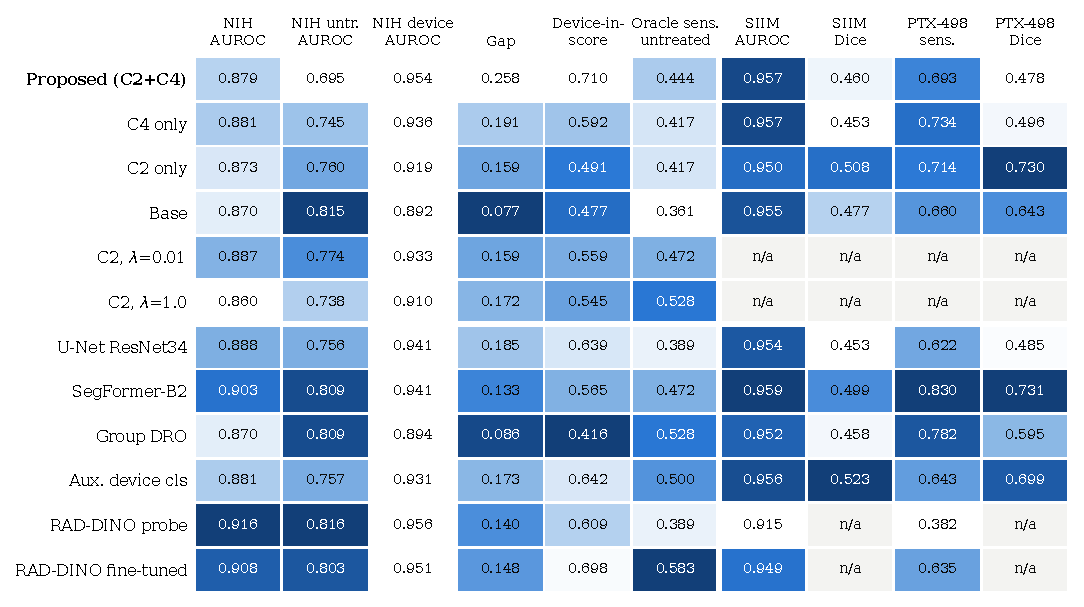
\includegraphics[width=\linewidth]{figures/fig_heatmap.pdf}
\caption{Model $\times$ metric overview. Cells show point estimates; colour encodes the within-column rank (darker = better; for the gap and device-in-score, lower is better). The NIH device-positive AUROC column is left uncoloured because a higher value there can reflect the shortcut. ``Oracle sens.\ untreated'' uses a threshold recalibrated on NIH at 95\% specificity. n/a: not computed for the sensitivity runs or no segmentation output.}
\label{fig:heatmap}
\end{figure}

\subsection{Device probe and leakage audit}
\label{sec:res-sanity}
The proposed model's pooled features still predicted device status on the NIH test set with a probe AUROC of 0.900. This was lower than for the auxiliary device classifier (0.973) and both RAD-DINO models (0.965, 0.960), but higher than for U-Net ResNet34 (0.845) and SegFormer-B2 (0.885). The adversary therefore did not remove device information from the representation.

The leakage audit found zero patient overlap between SIIM-ACR splits but four cross-split near-duplicate pairs. All four lie within the NIH cohort's own released splits. Three pair an NIH \emph{pilot-training} image with an NIH \emph{test} image, and one pairs an NIH \emph{pilot-validation} image with PTX-498 image SiteA\_98. None involves SIIM-ACR training or validation data, and the NIH pilot splits were used only to train the device classifier. The three NIH test images are all pneumothorax-negative. Excluding them left every estimate unchanged to the third decimal (the proposed model's untreated AUROC stayed at 0.695 and its gap moved from 0.258 to 0.259).

\subsection{Training dynamics}
\label{sec:res-conv}
\Cref{fig:convergence} shows per-epoch training and validation curves (mean and min--max over seeds). Training classification loss fell steadily to $10^{-2}$--$10^{-3}$ for the EfficientNet-B4 variants and the fine-tuned RAD-DINO, while validation AUROC reached 0.93--0.96, mostly within the first few epochs, and changed little afterwards (Group DRO declined to 0.91). Validation untreated sensitivity on SIIM-ACR reached 0.72--0.79 for the EfficientNet-B4 variants and 0.79 for SegFormer-B2, far above the 0.08--0.31 per-seed values observed at the same thresholds on NIH (\cref{fig:seeds}). Its min--max band was wide, reflecting the 32 untreated validation positives, and the epoch selected by \cref{line:select} of \cref{alg:train} varied from 2 to 14 across the proposed model's seeds. Validation Dice peaked early (about 0.50--0.54) and then drifted down slightly.

The device head behaved differently from what the design intended (\cref{fig:auxloss}b). In the proposed model the adversary's loss fell from 0.88 to 0.61 within three epochs and then stayed at the chance level of 0.60 (the label entropy for a batch device prevalence of about 0.71 under 50\% positive sampling). The encoder had therefore made $h$ uninformative \emph{to the adversary} on the development data. With the global head, adversarial losses stayed below chance for $\lambda=0.01$ (0.55) and $\lambda=0.1$ (0.58) and reached it only for $\lambda=1$. Without gradient reversal, the auxiliary device classifier drove its loss to nearly zero, confirming that device status is easy to read from the same features. Yet on NIH, device information remained linearly recoverable from the proposed model's $h$ (probe AUROC 0.900), and its score carried the strongest device signal of all models (device-in-score 0.710).

\begin{figure}[!tbp]
\centering
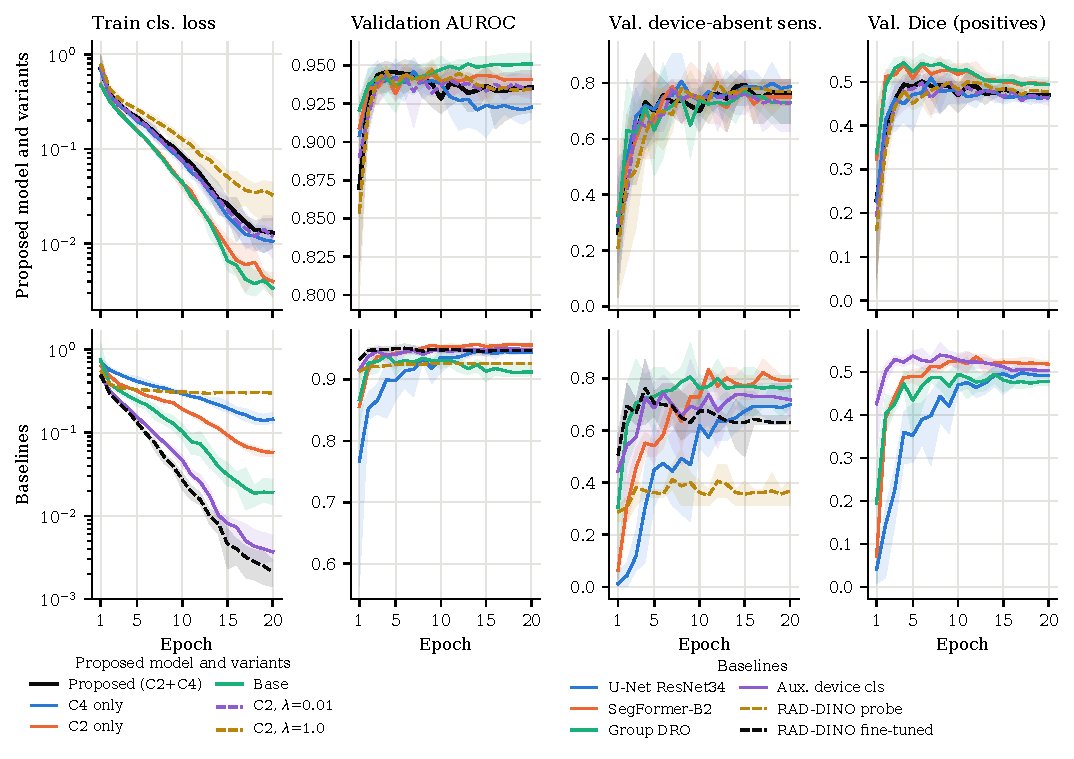
\includegraphics[width=\linewidth]{figures/fig_convergence.pdf}
\caption{Convergence curves on SIIM-ACR (mean with min--max band over 3--5 seeds). Top: proposed model, ablations and sensitivity variants; bottom: baselines. Training classification loss is on a log scale. Validation untreated sensitivity is computed at each epoch's own 95\%-specificity threshold on 32 untreated validation positives; it is the checkpoint-selection criterion of \cref{alg:train}. RAD-DINO models have no segmentation output.}
\label{fig:convergence}
\end{figure}

\begin{figure}[!tbp]
\centering
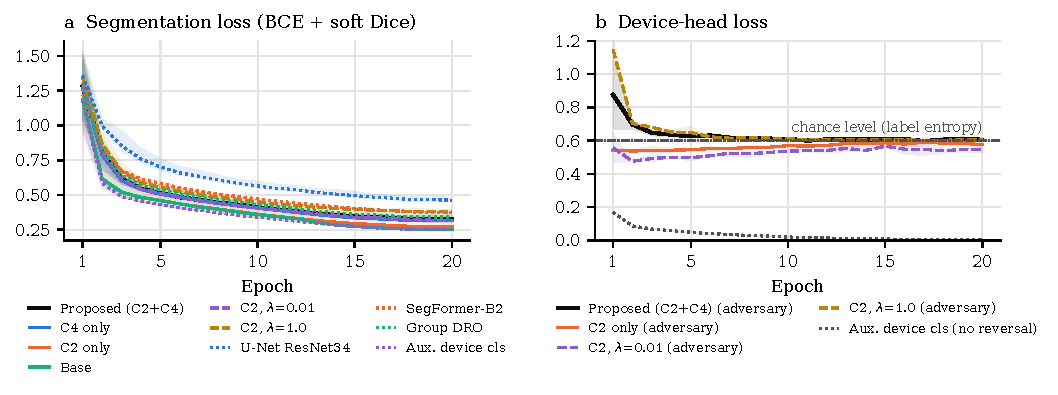
\includegraphics[width=\linewidth]{figures/fig_aux_losses.pdf}
\caption{Auxiliary training losses (mean with min--max band). (a) Segmentation loss (\cref{eq:lseg}); dotted lines are baselines. (b) Device-head loss: the adversary of \cref{eq:ladv} for C2 variants, and the auxiliary device classifier without reversal (logged with its loss weight 0.5). The dash-dotted line is the chance level, the entropy of the device label in training batches.}
\label{fig:auxloss}
\end{figure}

\subsection{Ablations and sensitivity runs}
\label{sec:res-ablation}
Neither component improved untreated sensitivity (\cref{tab:ablation}). Removing the adversary (C4 only) \emph{raised} mean untreated sensitivity from 0.206 to 0.256 and lowered the AUC gap from 0.258 to 0.191. Removing both components (base) gave the second-smallest gap of all models (0.077) and one of the highest untreated AUROCs (0.815). Among the C2 variants with a global head, $\lambda$ did not produce a monotone improvement (gap 0.159, 0.159 and 0.172 for $\lambda$ = 0.01, 0.1 and 1.0).

\begin{table}[!tbp]
\centering\small
\caption{Ablations on the NIH test set. Untreated sensitivity at the transferred threshold, mean over 5 seeds; ``seeds with drop'' counts paired seeds in which removing the component lowered the metric. Difference = full minus ablated, seed-averaged scores.}
\label{tab:ablation}
\begin{tabular}{@{}l l c c c c@{}}
\toprule
Ablation & Removed & Full & Ablated & Seeds with drop & Diff.\ (seed-avg) \ci{95\%}{CI} \\
\midrule
C4 only & C2 adversary & 0.206 & 0.256 & 1/5 & $-$0.028 \ci{$-$0.095}{0.000} \\
C2 only & C4 mask pooling & 0.206 & 0.211 & 2/5 & $-$0.056 \ci{$-$0.147}{0.000} \\
Base & C2 and C4 & 0.206 & 0.206 & 3/5 & $-$0.028 \ci{$-$0.095}{0.000} \\
\bottomrule
\end{tabular}
\end{table}

\subsection{The device shortcut across architectures (exploratory)}
\label{sec:res-shortcut}
Every configuration detected device-present pneumothorax better than untreated pneumothorax (\cref{fig:shortcut}a; \cref{tab:nih}). Point estimates of the gap ranged from 0.077 (base) to 0.258 (proposed). The gap's CI excluded zero for ten of twelve configurations; the exceptions were base and Group DRO. The radiology foundation model was not immune: RAD-DINO had the highest overall AUROC (0.916), yet its gap was 0.140 when frozen and 0.148 when fine-tuned.

The score-level analysis (\cref{fig:shortcut}c) shows the mechanism directly. Among pneumothorax-negative NIH radiographs, a device alone raised the pneumothorax score in eight of twelve configurations (\cref{eq:devscore} between 0.56 and 0.71, CI excluding 0.5). The proposed model had the strongest effect (0.710, 95\% CI 0.66--0.76). The configurations without this effect were base (0.477), Group DRO (0.416), C2 only (0.491) and the $\lambda$=1.0 variant (0.545, CI including 0.5).

In paired comparisons (\cref{fig:paired}), the proposed model's untreated AUROC was lower than that of base, Group DRO, SegFormer-B2, both RAD-DINO models and the $\lambda$=0.01 variant, with CIs excluding zero. Its gap was larger than that of eight of eleven comparators, again with CIs excluding zero.

\begin{figure}[!tbp]
\centering
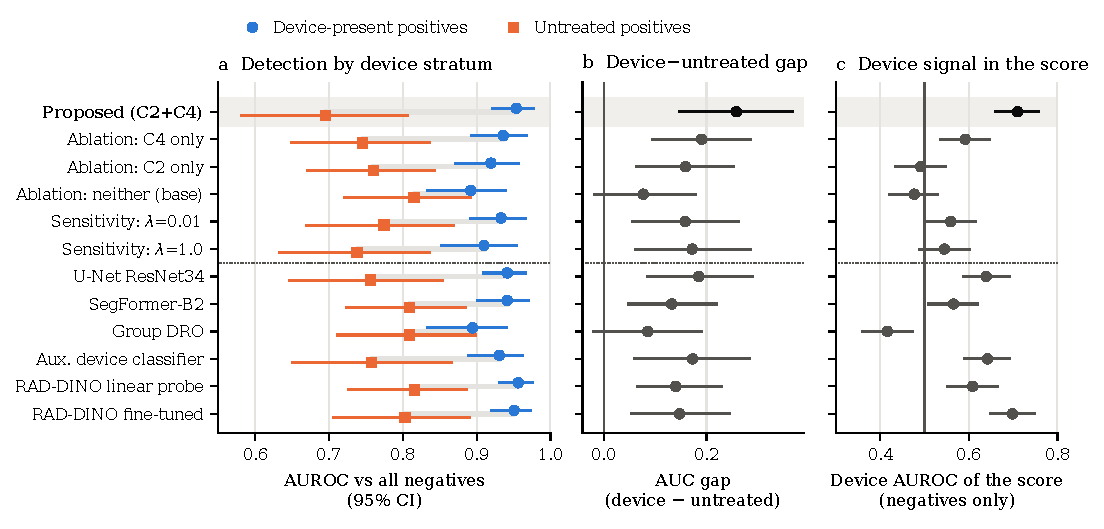
\includegraphics[width=\linewidth]{figures/fig2_shortcut.pdf}
\caption{Device shortcut on the NIH test set (seed-averaged scores; 95\% patient-cluster bootstrap CIs). (a) AUROC for device-present versus untreated pneumothorax against all negatives. (b) The gap between them (\cref{eq:gap}; primary endpoint). (c) Device AUROC of the pneumothorax score among pneumothorax-negative images (\cref{eq:devscore}); values above 0.5 mean a device alone raises the score. The dotted line separates the proposed model and its variants from the baselines.}
\label{fig:shortcut}
\end{figure}

\begin{figure}[!tbp]
\centering
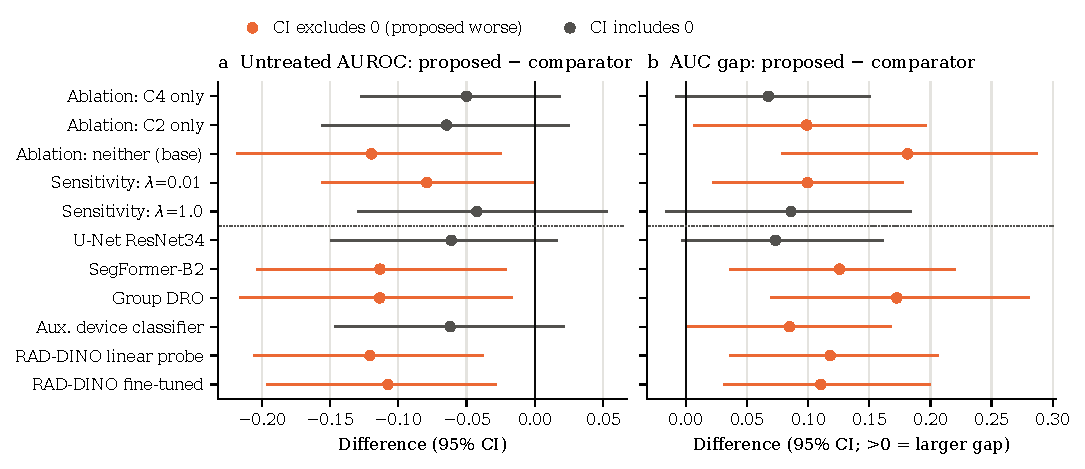
\includegraphics[width=\linewidth]{figures/fig3_paired.pdf}
\caption{Paired bootstrap differences between the proposed model and each comparator on the NIH test set (exploratory; shared resamples, \cref{alg:boot}). Orange marks CIs that exclude zero in the direction unfavourable to the proposed model.}
\label{fig:paired}
\end{figure}

\begin{figure}[!tbp]
\centering
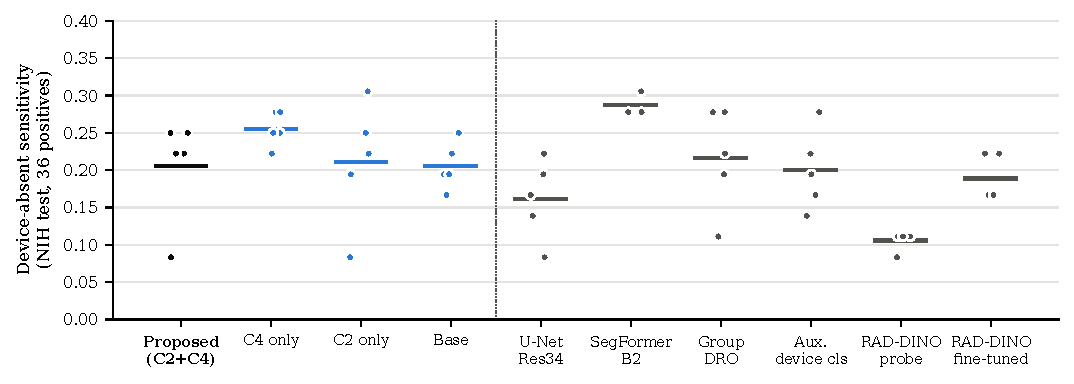
\includegraphics[width=\linewidth]{figures/fig4_seeds.pdf}
\caption{Per-seed untreated sensitivity on the NIH test set at the threshold transferred from SIIM-ACR validation (36 untreated positives, so one case = 0.028). Bars show seed means.}
\label{fig:seeds}
\end{figure}

\subsection{Operating-point transfer (exploratory)}
\label{sec:res-threshold}
Thresholds set at 95\% specificity on SIIM-ACR validation were far too strict on NIH. Specificity was 0.992--1.000 for every model, and overall sensitivity only 0.40--0.49. With a threshold recalibrated at 95\% specificity on the NIH set itself (an oracle, not a valid clinical estimate), overall sensitivity rose to 0.65--0.75 and untreated sensitivity to 0.36--0.58. The proposed model reached 0.744 overall and 0.444 untreated; the fine-tuned RAD-DINO model had the highest untreated value (0.583). Untreated sensitivity was therefore low in every model at every threshold considered.

\subsection{Example images and model maps (exploratory)}
\label{sec:res-qual}
Examples were chosen by rules fixed in the rendering script before any image was viewed, using the proposed model's seed-averaged NIH scores: the untreated positive with the highest score (untreated TP), the untreated positive with the lowest score (untreated FN), the device-present positive with the median score, the device-present \emph{negative} with the highest score (a shortcut candidate), and a device-free negative with the median score; plus two random SIIM-ACR internal-test positives with masks and one random PTX-498 image per site (random seed 0). For each model we averaged over seeds the segmentation probability $\sigma(Z)$ and Grad-CAM \citep{selvaraju2020gradcam} of the image logit $s(x)$ on the last encoder stage.

\Cref{fig:examples} shows the selected images and \cref{fig:maps} the seed-averaged maps for five models. The untreated positive with the highest score has a visible apical pneumothorax, and every model segmented it and scored it high (seed-averaged probability 0.86--1.00). The untreated positive with the lowest score is a device-free film on which the pneumothorax is not apparent at figure resolution; every model missed it (probability $\le$0.09), with no segmentation response and diffuse Grad-CAM. In the device-bearing \emph{negative} with the highest proposed-model score, several lines and ECG leads cross the chest. The proposed model, C4 only, SegFormer-B2 and Group DRO all placed pneumothorax probability over an upper zone crossed by these lines (probabilities 0.37--0.87), whereas the base model responded weakly (0.20). This single case matches the score-level result (\cref{eq:devscore}): the mask-pooling models convert device-related structures into ``pneumothorax pixels'', and the global-head base model does so least. It is an illustration, not evidence; the quantitative test is \cref{tab:nih}.

\IfFileExists{figures/fig_examples.pdf}{%
\begin{figure}[!tbp]
\centering
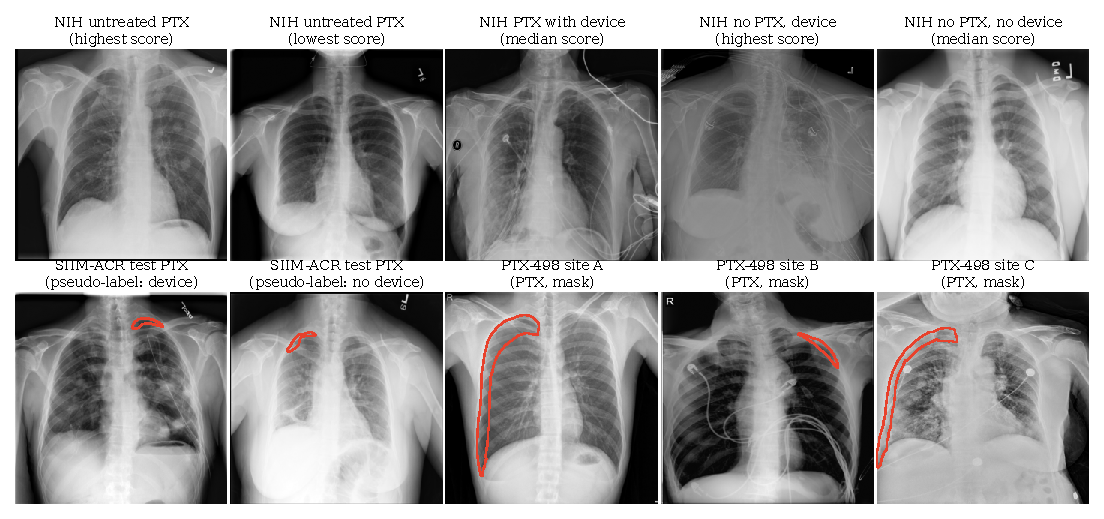
\includegraphics[width=\linewidth]{figures/fig_examples.pdf}
\caption{Example radiographs from each dataset with reference pneumothorax masks where available (red outline). NIH images are labelled with the human device annotation. Examples were chosen by fixed rules (\cref{sec:res-qual}).}
\label{fig:examples}
\end{figure}}{}

\IfFileExists{figures/fig_maps.pdf}{%
\begin{figure}[!tbp]
\centering
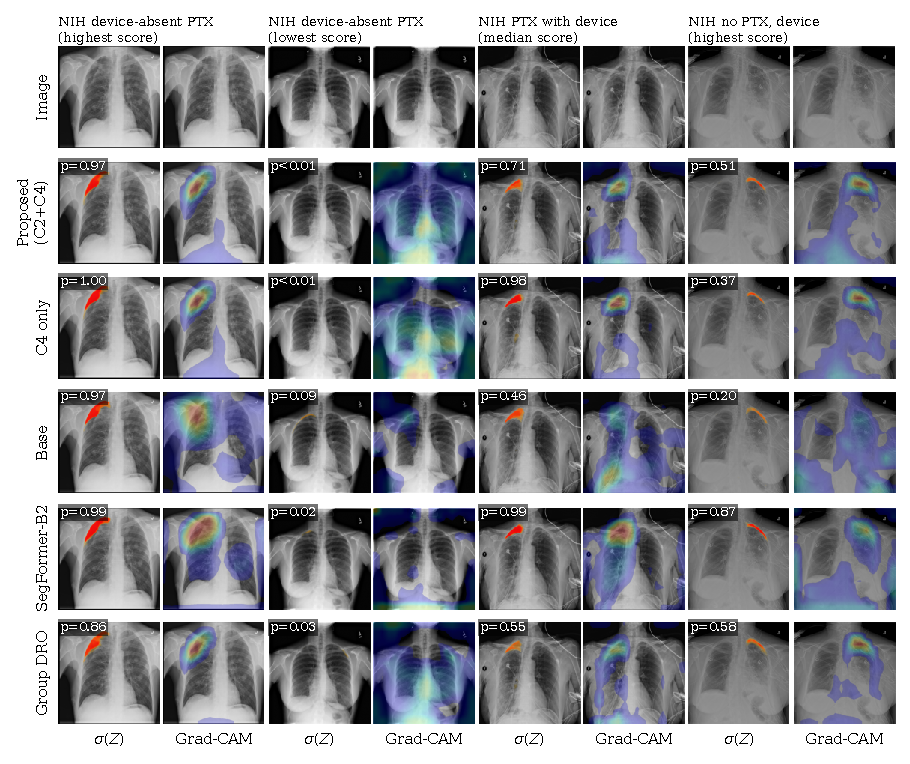
\includegraphics[width=\linewidth]{figures/fig_maps.pdf}
\caption{Seed-averaged model maps on the four NIH test cases selected by fixed rules. For each case, the left column shows the pneumothorax probability map $\sigma(Z)$ (red, opacity proportional to probability) and the right column Grad-CAM of the image logit $s(x)$. Numbers are seed-averaged predicted probabilities. Rows are models; the base model uses the global head, so its score does not depend on $\sigma(Z)$. Maps are illustrations only (see \cref{sec:discussion}).}
\label{fig:maps}
\end{figure}}{}


%% ============================================================ DISCUSSION
\section{Discussion}
\label{sec:discussion}

The hypothesis was not supported. A U-Net with a gradient-reversal device adversary and segmentation-based mask pooling, trained on SIIM-ACR with device pseudo-labels, was worse than simple baselines at detecting untreated pneumothorax on external data, and it had the largest device--untreated gap of the twelve configurations. The result is not borderline: both primary endpoints favoured the baselines, the ablations point in the unfavourable direction, and the exploratory paired analyses agree.

\paragraph{Why the deconfounding failed}
Several explanations are consistent with the data; the design cannot fully separate them.
\begin{enumerate}
  \item \emph{The adversary constrained the wrong pathway.} The adversary acted on globally pooled encoder features $h$, whereas C4 computes the decision from the decoder's segmentation logits $Z$ (\cref{fig:arch}). The training curves show that the adversary was driven to chance (\cref{fig:auxloss}b), so on the development data $h$ was uninformative to that particular head. The segmentation pathway, which bypasses $h$ through skip connections, was unconstrained. Consistent with this, C2 with a global head (whose score \emph{is} a function of $h$) had a device-in-score AUROC near 0.5, whereas C2 with C4 had the highest value observed. An adversary at chance is therefore not evidence of invariance: a linear probe on the same features still recovered device status externally (AUROC 0.900). This echoes benchmark findings that latent-space analyses reveal differences that task metrics miss \citep{muller2026disentangle}.
  \item \emph{Proxy mismatch and label noise.} The adversary targeted ``any visible device'' predicted by a classifier, not the chest tube. Pacemakers, lines and ECG leads are common in negatives (55\% of SIIM-ACR negatives were labelled device-bearing), so removing ``device'' information is not the same as removing ``tube'' information. Worst-group performance with inferred groups is known to trail that with oracle groups \citep{han2024gic,liu2021jtt}; our pseudo-labels were accurate on NIH validation (AUROC 0.98), but the relevant confounder is narrower than the label.
  \item \emph{Noisy model selection.} Checkpoints were selected on untreated sensitivity in a validation set with only 32 untreated positives, where one case moves the metric by 3 percentage points. The selected epochs ranged from 2 to 14 across seeds (\cref{fig:convergence}), and a validation value of about 0.76 fell to about 0.2 externally. The pilot's apparent advantage for C2+C4 on this criterion did not replicate.
\end{enumerate}
Simple baselines without attribute-specific machinery (base, Group DRO) had the smallest gaps and near-chance device-in-score values. Removing a shortcut in one distribution does not guarantee better behaviour in another \citep{yang2024limits}, and here the more elaborate debiasing made external behaviour worse.

\paragraph{The shortcut is general}
Across convolutional, transformer and foundation-model backbones, every model found device-present pneumothorax easier, and in most the score itself carried device information that a clinician would not want in a pneumothorax detector. This agrees with reports that thoracic tubes confound pneumothorax algorithms \citep{rueckel2020tubes,rueckel2021annotations}, with saliency evidence of tube bias \citep{wollek2023attention}, with the lower performance of CLIP-based models on drain-free images \citep{sourget2025clip}, and with foundation encoders using tube shortcuts \citep{li2025featurequality}. It contrasts with studies that found no tube effect \citep{thian2021external,seah2021hidden,graf2020tube}. Those models were trained on larger or differently labelled data, used lung segmentation, or tested tube-bearing \emph{positives} against all negatives; the stratum that separates the hypotheses, device-bearing negatives, was rarely analysed. Our device-in-score metric (\cref{eq:devscore}) isolates that stratum and requires only device labels on the test set. Overall AUROC hides the problem: RAD-DINO had the highest overall AUROC and a clear gap. We therefore recommend that pneumothorax studies report untreated-stratum AUROC and the device-in-score AUROC as standard.

\paragraph{What the heatmaps can and cannot show}
The qualitative maps in \cref{sec:res-qual} are illustrations chosen by fixed rules, not evidence. Saliency methods localise poorly on chest radiographs and can fail sanity checks \citep{saporta2022saliency,arun2021saliency}. For the mask-pooling models the segmentation probability map is the more faithful view, because it is the quantity from which the score is computed (\cref{eq:maskpool}). The quantitative evidence for the shortcut is the stratified AUROCs and the score-level test, not the maps.

\paragraph{Threshold transfer}
A 95\%-specificity threshold chosen on SIIM-ACR gave near-100\% specificity and under 50\% sensitivity on NIH for every model. Any clinical deployment would require local recalibration. It also explains why untreated sensitivity at the transferred threshold is low and compressed across models.

\paragraph{Limitations}
The primary external set contains only 36 untreated positives, so untreated sensitivity has coarse resolution and wide CIs. Plan B used device pseudo-labels rather than chest-tube masks, so this study does not test the original hypothesis with tube-specific components (inpainting, auxiliary tube segmentation); that remains open. SIIM-ACR and the NIH cohort both derive from ChestX-ray14; we removed near-duplicates at image level, but patient-level overlap cannot be excluded. SegFormer-B2 and the sensitivity runs used three seeds rather than five. nnU-Net and zero-shot multimodal models were not evaluated. Four near-duplicate pairs inside the NIH cohort's own released splits were found; excluding them changed no estimate.

\paragraph{Implications for method design}
Three changes follow from the training dynamics. First, a debiasing constraint should act on the pathway that produces the score: for mask pooling, on decoder features or on $Z$ itself, for example by penalising the dependence of $s(x)$ on the device among negatives. Second, adversary loss at chance should not be read as success; a held-out probe should be monitored during training. Third, pixel-level supervision of the pleural line \citep{rueckel2021annotations} or counterfactual editing of devices \citep{cooke2026roentmod} target the confounder directly and may be more promising than representation-level adversaries with proxy labels.

\paragraph{Value of pre-registration}
The pilot on SIIM-ACR validation suggested a gain of 3--12 percentage points in untreated sensitivity for the proposed model. Without a frozen external protocol it would have been easy to report internal results, adjust thresholds on the external set, or choose a favourable subset of metrics. Freezing endpoints and opening external data once (\cref{alg:eval}, \cref{line:hash}) made the negative result unambiguous.

%% ============================================================ CONCLUSION
\section{Conclusion}
\label{sec:conclusion}
Gradient-reversal deconfounding with pseudo-labelled device information did not help a segmentation-pooled pneumothorax detector find untreated pneumothorax. On external data with human device labels it increased the model's reliance on devices, even though the adversary was driven to chance during training. All twelve configurations, including a radiology foundation model, showed a device shortcut, and thresholds did not transfer between public datasets. Future work should use true chest-tube annotations, constrain the pathway that produces the score, select checkpoints on larger untreated validation sets, and report untreated-stratum and device-in-score metrics as standard.

\section*{Data and code availability}
Code, configuration files, frozen split files, the pre-registration and its hash, per-image predictions for every run and dataset, per-epoch training logs and the evaluation report are in the project repository (\url{https://github.com/yazanjer/ptx-deconfound}; public at publication). All 54 model checkpoints are archived on Zenodo together with a manifest (SHA-256 and MD5 checksums, run, seed and 95\%-specificity threshold for each file) and a model card (\url{https://doi.org/10.5281/zenodo.22966372}); they are also release assets of the repository (\texttt{weights-v1}). Source images are not redistributed. SIIM-ACR and NIH ChestX-ray14 are available from Kaggle; the NIH device cohort manifest \citep{zamora2026cohort} and PTX-498 \citep{wang2021ptx498} are available from Zenodo.

\section*{Deviations from the pre-registration}
\begin{enumerate}
  \item Amendment~1 (Plan B) replaced CANDID-PTX with SIIM-ACR as the development set and chest-tube labels with device pseudo-labels, because CANDID-PTX could not be accessed. It was recorded before any external evaluation.
  \item nnU-Net and zero-shot multimodal baselines were not run, and tube-mask components were dropped. This was recorded before freezing.
  \item Infrastructure events with no effect on endpoints: two U-Net ResNet34 seeds were re-trained after a result-upload failure; the first RAD-DINO attempt stopped at model loading and was re-run unchanged; one run's configuration file (identical across seeds) was restored after it was lost in a concurrent upload. No external set was opened during any of these.
  \item The convergence curves, heatmap overview and qualitative maps (\cref{sec:res-conv,sec:res-qual}) were produced after the external evaluation, from stored logs and checkpoints; they involve no training, tuning or new metrics on the endpoints.
\end{enumerate}

\section*{Declaration of generative AI and AI-assisted technologies in the manuscript preparation process}
During the preparation of this work the author used Claude (Anthropic) to assist with code development, experiment orchestration, statistical analysis, literature search and manuscript drafting. After using this tool, the author reviewed and edited the content as needed and takes full responsibility for the content of the published article.

\section*{Ethics statement}
This study used only publicly available, de-identified datasets (SIIM-ACR, NIH ChestX-ray14 and the derived device cohort, PTX-498) under their respective licences. No new patient data were collected. [Author to confirm whether institutional review-board exemption applies.]

\section*{CRediT authorship contribution statement}
\textbf{Yazan Aljeroudi:} Conceptualization, Methodology, Software, Formal analysis, Investigation, Data curation, Visualization, Writing -- original draft, Writing -- review \& editing.

\section*{Declaration of competing interest}
The author declares no competing interests.

\section*{Funding}
[To be completed by the author.]

\bibliographystyle{elsarticle-num-names}
\bibliography{refs}

\end{document}
